\documentclass{standalone}
\usepackage[T1]{fontenc}\usepackage{tikz}
\usepackage{amsmath, amsfonts}
\usetikzlibrary{arrows.meta}
\begin{document}
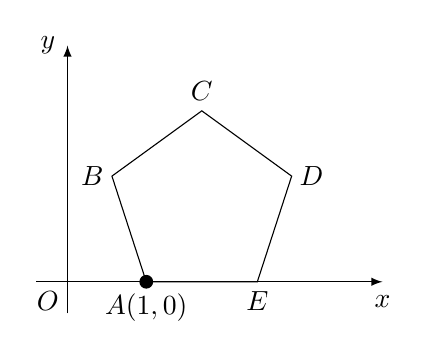
\begin{tikzpicture}
\draw[] (0.000000, 1.200000) -- (-1.141268, 0.370820) -- (-0.705342, -0.970820) -- (0.705342, -0.970820) -- (1.141268, 0.370820) -- cycle;
\node[] at (0.000000,1.450000) {$C$};
\node[] at (-1.391268,0.370820) {$B$};
\node[] at (-0.705342,-1.300820) {$A(1, 0)$};
\node[] at (0.705342,-1.220820) {$E$};
\node[] at (1.391268,0.370820) {$D$};
\draw[fill=black, draw=black] (-0.705342, -0.970820) circle (0.080000);
\node[] at (2.294658,-1.220820) {$x$};
\node[] at (-1.955342,2.029180) {$y$};
\node[] at (-1.955342,-1.220820) {$O$};
\draw[-latex] (-2.105342, -0.970820) -- (2.294658, -0.970820);
\draw[-latex] (-1.705342, -1.370820) -- (-1.705342, 2.029180);
\end{tikzpicture}
\end{document}
